\documentclass[12pt]{beamer}

\usepackage[size = a0, orientation = portrait, scale = 1.5]{beamerposter}

\usefonttheme{serif}

\usepackage[english]{babel}
\usepackage[utf8x]{inputenc}
\usepackage[T1]{fontenc}
\usepackage{lmodern}
\usepackage{indentfirst}
\usepackage{ragged2e}
\usepackage[]{natbib} 
\usepackage{graphicx}
\usepackage{animate}
\usepackage{color}
\usepackage{colortbl}

% For 'InkScape' integration
\usepackage{import}
\usepackage{xifthen}
\usepackage{pdfpages}
\usepackage{transparent}

\setbeamertemplate{navigation symbols}{}
\setbeamertemplate{caption}[numbered]

\definecolor{title-bg}{RGB}{240, 240, 240}
\definecolor{title-fg}{RGB}{128, 113, 93}
\definecolor{my-red}{RGB}{254, 132, 135}
\definecolor{my-blue}{RGB}{59, 180, 252}
\definecolor{my-green}{RGB}{125, 221, 149}
\definecolor{titles}{RGB}{0, 166, 160}
\setbeamercolor{block title}{fg = title-fg, bg = title-bg}
\setbeamercolor{header-color}{fg = title-fg, bg = title-bg}

\setbeamertemplate{headline}{%
\begin{beamercolorbox}[wd=1.00\textwidth]{header-color}
	\begin{columns}[T]
		\begin{column}{0.235\textwidth}
			
\includegraphics[width=1.15\linewidth]{Images/KAUST_logo} 
		\end{column}
		\begin{column}{0.630\textwidth}
			\vspace{32pt}
			\begin{beamercolorbox}[wd=1.00\textwidth]{header-color}	
			{\Large Assessing the Effect of Model-based Geostatistics Under Preferential Sampling for Spatial Data Analysis \par} \vspace{12pt}
			
			{\normalsize
				André Victor Ribeiro Amaral${\phantom{|}}^{1, \star}$, 
				Paula Moraga${\phantom{|}}^{1}$
			}	\vspace{16pt}
		
			{\footnotesize
			${}^{1}\hspace{8pt}$Computer, Electrical and Mathematical Sciences and Engineering Division, King Abdullah University of Science and Technology (KAUST).  \\ \vspace{3pt}
			${}^{\star}$ E-mail: \texttt{andre.ribeiroamaral@kaust.edu.sa}
			}
			\end{beamercolorbox}
			\vspace{24pt}
		\end{column}
		\begin{column}{0.135\textwidth}
		\vspace{25pt}
		
\includegraphics[width=0.85\linewidth]{Images/METMAX_logo}
		\end{column}
	\end{columns}
\end{beamercolorbox}
}
\setbeamertemplate{footline}{}

\begin{document}
	\begin{frame}[t]
		\begin{columns}[t]
			%======================================== FIRST COLUMN ========================================
			\begin{column}{0.30\textwidth} \justifying % FIRST COLUMN
			\begin{block}{\Large 1. Introduction} \justifying \vspace{12pt}				

			For problems from the geostatistics domain, it is usually assumed that the sampling process is independent of the process of interest. However, this may not always be the case, and in situations where this assumption does not hold, we say we have \textit{preferential sampling}, as in \cite{diggle2010geostatistical}.\vspace{18pt}
			
			%Aiming to accommodate the dependence between the sampling process and the process of interest into the modeling approach, and methods that take this dependence into account to obtain valid inferences have been developed \cite{diggle2010geostatistical, dinsdale2018methods, pati2011bayesian}.\vspace{18pt}
			
			Before, models that account for preferential sampling were fitted by rewriting the likelihood function in a way that it could be seen as an expectation, allowing researchers to approximate it by Monte Carlo methods. However, more recently, a Bayesian approach relying on the Integrated Nested Laplace Approximation (INLA) and Stochastic Partial Differential Equation (SPDE) methods started to be employed.\vspace{18pt}
			
			\end{block}
		
			\begin{block}{\Large 2. Geostatistical Model} \justifying \vspace{12pt}				
				
				%Let $X = (X_1, \cdots, X_n)$, $n \in \mathbb{N}$, be a random vector, such that $x_i \in \mathcal{A} \subseteq \mathbb{R}^2$, $\forall i$, and let $S$ be a real-valued stochastic process, such that $S(X) = (S(X_1), \cdots, S(X_n))$ is a discrete set of observations of $S$ evaluated at $X$. In that way, if $[S, X] \neq [S][X]$, then we say we are under a  \textit{preferential sampling} setting.\vspace{18pt}
				
				
				A geostatistical model to predict a spatially continuous process can be defined as follows. 
				Suppose that $Y_i$ denotes the observed value of a noisy version of a spatial process $S(x_i)$ at some given location $x_i \in \mathcal{A} \subseteq \mathbb{R}^2$, for $i \in \{1, \cdots, n\}$, in the following manner
				\begin{align} \label{eq:main-model}
					Y_i = \mu + S(x_i) + \epsilon_i,
				\end{align}
				where $\epsilon_i$ are independent Gaussian zero-mean random variables with $\text{Var}(\epsilon_i) = \sigma^2_{\epsilon}$. Also, $S(x_i)$ will be assumed to have zero mean---meaning that $\mathbb{E}(Y_i) = \mu$, $\forall i$.\vspace{18pt}
				
				Additionally, let $x = (x_1, \cdots, x_n)$ be a realization of a random vector  $X = (X_1, \cdots, X_n)$ and $S(x) = (S(x_1), \cdots, S(x_n))$ a realization of a random process $S(X) = (S(X_1), \cdots, S(X_n))$ evaluated at $X$. In this case, although Model \eqref{eq:main-model} is fairly common, it usually assumes that $X$ is stochastically independent from $S(X)$, which is not reasonable in many situations.\vspace{18pt}
				
				To account for this dependence, as in \cite{diggle2010geostatistical}, the following additional assumptions for Model \eqref{eq:main-model} are required\vspace{18pt}
				\begin{enumerate} \justifying
					\item $S$ is a stationary and isotropic Gaussian random field with mean zero, variance $\sigma^2$, and correlation function $r(h; \theta) = \text{corr}(S(x_1), S(x_2))$, for $h \neq 0$, where $h$ is the Euclidean distance between $x_1$ and $x_2$.
					\item $X|S \sim \text{Poisson Process}(\lambda(x))$ with intensity $\lambda(x) = \exp\{\alpha + \beta S(x)\}$, for $\alpha, \beta \in \mathbb{R}$.
					\item Conditional on $S$ and $X$, the $Y = (Y_1, \cdots, Y_n)$ is a vector of independent Gaussian random variables, such that $Y_i \sim \text{Normal}(\mu + S(x_i), \sigma^2_{\epsilon})$, $\forall i$.
				\end{enumerate}\vspace{18pt}
				
			\end{block}
				
				
			\begin{block}{\Large 3. Inference} \justifying \vspace{12pt}				
				
				Since the original paper that introduced the preferential sampling idea was published by \cite{diggle2010geostatistical}, people have been working on this class of problems using different approaches. Here, we will present two of them, namely the original idea, and the a method that uses INLA and the SPDE techniques. 
				
			\end{block}
			
			\end{column}
		
			%======================================== SECOND COLUMN ========================================
			\begin{column}{0.30\textwidth} \justifying % SECOND COLUMN
			
			{\large \textcolor{title-fg}{Original Approach}} \vspace{18pt}
				
			Start by recalling that, if we consider Model \eqref{eq:main-model} and if we want to predict the value of the process in, say, $x_0$, we can use, for instance, the Best Unbiased Linear Predictor (BLUP). And to do this, we have to be able to estimate the parameters of the model. In particular, if $S(x)$ is a Gaussian random field with a covariance structure described by $\Sigma(\theta)$, this can be done through the Maximum Likelihood method.\vspace{18pt}
			
			In that case, if $X$ and $S(X)$ are not independent, then the likelihood function $\mathcal{L}(\theta)$, given the data, is
			\begin{align} \label{eq:main-likelihood}
				\mathcal{L}(\theta) = [X, Y] &= \displaystyle\raisebox{-18pt}{\scalebox{3.2}{\ensuremath{\int}}} [X, Y, S] dS \nonumber \\
															   &= \displaystyle\raisebox{-18pt}{\scalebox{3.2}{\ensuremath{\int}}} [Y|S, X][X|S][S]dS.
			\end{align}
		
			\vspace{6pt}
			Therefore, to determine $\theta$ that maximizes $\mathcal{L}(\theta)$, one has to solve the integral in Equation \eqref{eq:main-likelihood}. And for this problem, \cite{diggle2010geostatistical} has proposed a way to approximate $\displaystyle\raisebox{-18pt}{\scalebox{3.2}{\ensuremath{\int}}} [Y|S, X][X|S][S]dS$ using a Monte Carlo method. Then, from the approximated likelihood function, they could do inference by determining $\theta$ that maximizes $\mathcal{L}_{\text{Approx.}}(\theta)$.\vspace{18pt}\vspace{18pt}
			
			{\large \textcolor{title-fg}{INLA and SPDE Approach}} \vspace{18pt}
			
			An alternative approach to estimate the model parameters and make prediction for Model \eqref{eq:main-model} is to use the INLA and SPDE approaches, which can be easily implemented with the \texttt{R-INLA} package \cite{rue2009approximate}.
			In a nutshell, INLA is a method for approximating Bayesian inference in latent Gaussian models \cite{moraga2019geospatial}. In particular, models are of the form
			\begin{align*}
				y_i|S(x_i), \theta &\sim \pi(y_i|S(x_i), \theta), \text{ for } i \in \{1, \cdots, n\} \\
				S(x)|\theta &\sim \text{Normal}(\mu(\theta), Q(\theta)^{-1}) \\
				\theta &\sim \pi(\theta),
			\end{align*}
			where $y = (y_1, \ldots, y_n)$ is the vector or observed values, $x = (x_1, \ldots, x_n)$ is a Gaussian random field, and $\theta = (\theta_1, \ldots, \theta_k)$, for some $k \in \mathbb{N}$, is a vector of hyperparameters. $\mu(\theta)$ and $Q(\theta)$ represent the mean vector and the precision matrix, respectively.\vspace{18pt}
			
			From the above formulation, notice that Model \eqref{eq:main-model} can be classified as a latent Gaussian model, and therefore we can use the INLA method. To fit Model \eqref{eq:main-model} model using \texttt{R-INLA}, we will take an SPDE approach. As showed in \cite{whittle1963stochastic}, a Gaussian random field with Mat\'{e}rn covariance matrix can be expressed as a solution of
			\begin{align*}
				(\kappa^2 - \Delta)^{\alpha/2}(\tau S(x)) = \mathcal{W}(x),
			\end{align*} 
			where $\Delta$ is the Laplacian, $\mathcal{W}(s)$ is a Gaussian white-noise random process, $\alpha$ controls the smoothness of the random field, $\tau$ controls the variance, and $\kappa$ is a scale parameter. Based on this, \cite{lindgren2011explicit} proposed a new approach to represent a Gaussian random field with Mat\'{e}rn covariance as a Gaussian Markov Random Field {\normalfont(GMRF)}, by representing a solution to the SPDE using the finite element method. This representation implies a sparse precision matrix for the spatial effects, allowing the implementation of fast computational methods to do inference.
			
			\end{column}
		
			%======================================== THIRD COLUMN ========================================
			\begin{column}{0.30\textwidth} \justifying % THIRD COLUMN
		
			\begin{block}{\Large 4. Simulation and Results} \justifying \vspace{12pt}				
				
			For $n = 100$ sampled locations $x_i$, we take measurements of the simulated processes $S$. In preferential sampling scenarios, points are a realization of $X|S \sim \text{Poisson Process}(\lambda(x))$, s.t. $\lambda(x) = \exp\{\alpha + \beta S(x)\}$ with $\beta > 0$.  However, in non-preferential sampling scenarios, $X \sim \text{Poisson Process}(\lambda(x))$ s.t.  $\lambda(x) = \exp\{\alpha\}$.\vspace{18pt}
			
			Different scenarios were considered, but here we will present just two; one for preferential sampling and another one for non-preferential sampling. In all cases, we set $\mu = 0$ and $\sigma^2_{\epsilon} = 1$. Then, after generating data, we fit Model \eqref{eq:main-model} under the assumption that $X$ and $S(X)$ are \textbf{independent} (\texttt{A1}) and \textbf{dependent} (\texttt{A2}).\vspace{18pt}
			
			For instance, Figure \ref{fig:threeplots} shows simulated scenario under preferential sampling and fitted models based \texttt{A1} and \texttt{A2}. Visual inspection suggests better results for model $\texttt{A2}$.\vspace{9pt}
			\begin{figure}[!htb] \label{fig:threeplots}
				\begin{center}
					{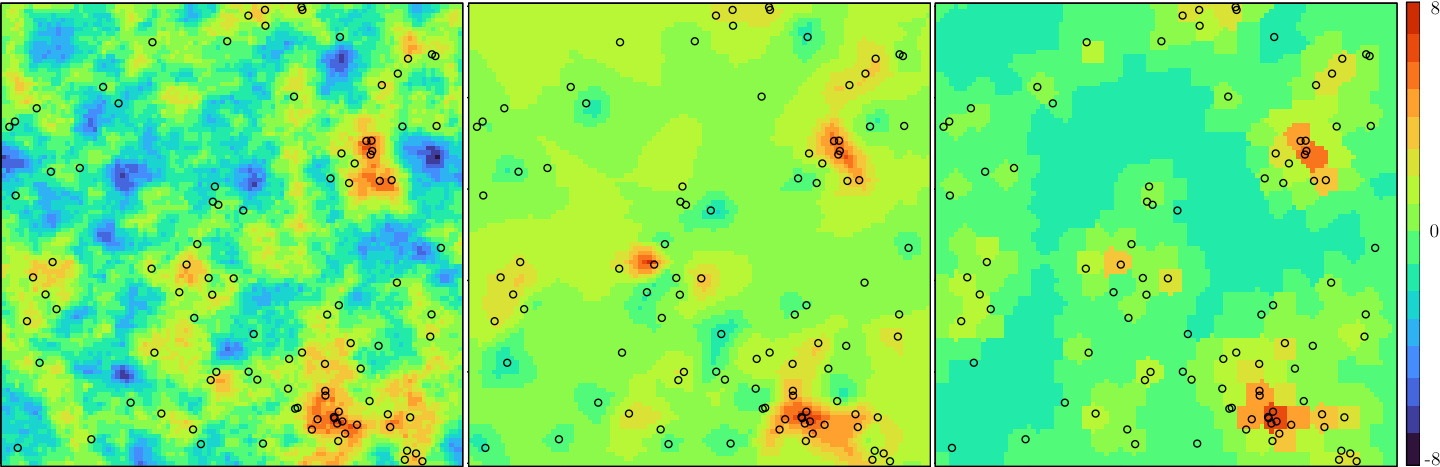
\includegraphics[width=1\textwidth]{Images/three_plots.png}}
					\caption{\justifying Simulated $S$ and $X|S$ processes (left) with estimation based on models \texttt{A1} (center) and \texttt{A2} (right).}
				\end{center}
			\end{figure}
				
			For the two simulated scenarios and the two fitted models, we assessed the performance of \texttt{A1} and \texttt{A2} by computing the Mean Squared Error (MSE). We simulated $m = 50$ data sets from each of the two scenarios and computed the mean and quantiles of the MSEs (Table \ref{tab:errors}).
			
			\vspace{-36pt}
			\begin{table}[!htb] \label{tab:errors}
				\begin{center}
					\resizebox{1\textwidth}{!}{%
						\begin{tabular}{c|c|c|c}
							\hline
							Scenario 									& Model 	  & Mean (SD) of $\text{MSE}$ 		   & $5^{\text{th}}$---$95^{\text{th}}$ perc. of $\text{MSE}$ \\ \hline
							Non-pref. sampl.  					 & \texttt{A1} & 3.16 (0.33) 									   & 2.70---3.75\\
							Non-pref. sampl.  					 & \texttt{A2} & 3.59 (0.48) 									 & 3.03---4.50\\
							Prefer. sampling\phantom{.}  & \texttt{A1} & 5.63 (1.07) 									  & 4.19---7.80 \\
							Prefer. sampling\phantom{.}  & \texttt{A2} & 3.44 (0.59) 									 & 2.80---4.80\\
							\hline
						\end{tabular}%
					}%
					\vspace{12pt}\caption{\justifying Computed statistics for the $\text{MSEs}$ for models $\texttt{A1}$ and $\texttt{A2}$ in the two scenarios.}
				\end{center}
			\end{table}
				
			From the table, for the scenario in which preferential sampling was \textbf{not} considered for the data generation procedure, $\texttt{A1}$ performed \textit{slightly} better than $\texttt{A2}$; however, for data generated with preferential sampling, model $\texttt{A2}$ performed \textit{much} better than model $\texttt{A1}$ (w.r.t. the MSE).\vspace{18pt}
				
			\end{block}
		
			\begin{block}{\Large 5. Conclusions} \justifying \vspace{12pt}				
				
				Careful consideration of the obtained data is needed in order to determine the most appropriate modeling approach in each situation. Sometimes, we will need to account for preferential sampling if the obtained sample depends on the underlying spatial process. In other situations, though, standard geostatistical models will suffice to obtain valid inferences.\vspace{18pt}
				
				% Thus, although preferential sampling may play an important role in the modeling procedure, careful consideration of the obtained data is required to determine the appropriate technique.\vspace{18pt}
				
			\end{block}
		
			
		
		
			\begin{block}{References}\justifying \vspace{12pt}\tiny
				\bibliographystyle{plain}
				\bibliography{References/References}
			\end{block}	
					
			\end{column}
		\end{columns}
	\end{frame}


\end{document}